\documentclass[letterpaper]{article}

\usepackage{hyperref}
\usepackage{geometry}
\usepackage{graphicx}
\usepackage{amsmath}
\usepackage{amssymb}
\usepackage{algorithmic}
\usepackage{algorithm}
\usepackage{tikz}
\usepackage{hhline}
\usepackage{multirow}
\usepackage{caption}
\usepackage{subcaption}

\setlength\parindent{0pt}

\begin{document}

\title{CS224N Neural Networks for Name Entity Recognition}
\author{
        Jiayuan Ma \\
        \texttt{jiayuanm@stanford.edu}
        \and
        Xincheng Zhang\\
        \texttt{xinchen2@stanford.edu}
}
\maketitle


\section{Implementation Details}

\subsection{Matlab Style Code}
Because we are comfortable with Matlab style of operating with matrices and vectors and EJML does not support all Matlab-like APIs, we choose to implement some Matlab style matrix helper functions such as \texttt{repmat}, \texttt{horzcat} in \texttt{MatlabAPI}.

\vspace{0.1cm}

We also implement several helper methods such as \texttt{sigmoid}, \texttt{tanh}, \texttt{tanhDerivative} to make our neural network code more modular, e.g. feedforward to be more readable.

\subsection{Multiple Layer Support}
Since we decide to target Extra Credit at the very beginning, our design and implementation automatically support multiple ($\ge 1$) hidden layer neural networks (or deep architectures). In addition to the default constructor of \texttt{WindowModel} which takes in a single number as the size of one hidden layer, the sizes of multiple hidden layers can be passed in as an array of integers to another ``deep'' constructor of \texttt{WindowModel}. All our implementations of feed forward propagation, back propagation and gradient checking support multiple layer architectures.  

\subsection{Building Blocks}

\textbf{Feed Forward}: The implementation of feed forward function is relatively straightforward: doing iterative matrix multiplications and feeding the result to  nonlinear activation functions ($\tanh$ or sigmoid depends on which layer we are processing). We also implemented a regularized likelihood cost function to analyze the changes of cost function during training.
We implemented these two functions in batch mode,
which can take in a batch of inputs, not a single input.
\begin{verbatim}
Line 235: public SimpleMatrix batchFeedforward(SimpleMatrix windows)
Line 251: public double costFunction(SimpleMatrix X, SimpleMatrix L)
\end{verbatim}

\textbf{Initialization}: We initialize all $W$ randomly and set $b$ to zero as instructed. In addition, since we support multiple layer, the $fanIn$ value of each deeper layer is the hidden size of its previous layer.
\begin{verbatim}
Line 280: public void initWeights()
\end{verbatim}
\textbf{Back Propagation}: There are several smaller components for building back propagation algorithm.
We first do a feed forward propagation to get $z^{(l)}$ and $a^{(l)}$ (defined in (\ref{eq:activation})), and then back propagate errors to calculate the gradient. We refer interested readers to Section \ref{sec:grad} for more details. The following implementation also supports gradient in batch mode so that we can also experiment with mini-batch gradient descent.
\begin{verbatim}
Line 313: protected SimpleMatrix[] backpropGrad(SimpleMatrix batch, SimpleMatrix label)
\end{verbatim}

\textbf{Gradient Check}: 
We implemented the numerical gradient calculation in
\begin{verbatim}
Line 418: protected SimpleMatrix[] numericalGrad(SimpleMatrix batch, SimpleMatrix label)
\end{verbatim}
and we use \texttt{checkGradient} function to ensure our gradient is calculated correctly (the $L_\infty$ norm between two gradient vectors is below $10^{-8}$).

\vspace{0.1cm}

All of these components are implemented to support multiple layers calculation as well as batch mode. We setup an initial run with window size ($C$) 5, one hidden layer of size ($H$) 100, iterations through the dataset ($K$) 20. The F1 score is 0.734.

 
\section{Gradients by Backpropagation (with Extra Credit)}\label{sec:grad}
First of all, we ``absorb'' all bias terms into their corresponding weight matrices.  We did this by appending bias terms as the first column of the new weight matrices and padding. Doing so simplifies the problem formulation and derivation of gradients.

For example, the procedure works as follows.
\begin{equation}
W x + b
\qquad
\textrm{ is rewritten into }
\qquad
W^\prime
x^\prime
=
\begin{bmatrix}
b & W
\end{bmatrix}
\begin{bmatrix}
1 \\ x
\end{bmatrix}
\end{equation}
Unless otherwise indicated, the report assumes the weight matrix $W^{(l)}$ of layer $l$ is the absorbed version of the original weight matrix and its corresponding bias term, i.e.
\begin{equation}
\begin{split}
W^{(l)} & =
\begin{bmatrix}
b^{(i)} & W^{(l)}_\textrm{ori}
\end{bmatrix} \\
U &=
\begin{bmatrix}
b & U_\textrm{ori}
\end{bmatrix}
\end{split}
\end{equation}


We derive the gradients of our neural network regardless
of how deep the network is. Therefore, the gradients derived here apply to networks of one or multiple hidden layers (extra credit).

\vspace{0.1cm}

For a network that has $L$ hidden layers, we iteratively define the activation vectors $a^{(l)}$ and each layer's nonlinear input vectors $z^{(l)}$ as follows.
\begin{equation}\label{eq:activation}
\begin{split}
z^{(0)} = x
& \qquad 
a^{(0)} =
\begin{bmatrix}
1 \\ z^{(0)}
\end{bmatrix} 
\qquad
\textrm{where } x \textrm{ is the input vector} \\
z^{(l)} = W^{(l)} a^{(l-1)}
& \qquad
a^{(l)} = 
\begin{bmatrix}
1 \\ f(z^{(l)})
\end{bmatrix}
\qquad
\textrm{for } l = 1, \dots, L \\
z^{(L+1)} = U a^{(L)}
& \qquad
a^{(L+1)} = g(z^{(L+1)})
\end{split}
\end{equation}
where $f$ is the nonlinear $\tanh$ function and $g$ is the sigmoid function. Notice that the definition of $a$ and $z$ follow closelt the procedure of forward propagation. The final layer of activation $h_\theta(x) = a^{(L+1)}$ is the output of the entire neural network.

\vspace{0.1cm}

Back propagation algorithm works by propagating errors $\delta^{(l)}$ progressively from the output layer to the input layer. Following back propagation, we give the iterative definition of $\delta^{(l)}$ as follows.
\begin{equation}
\begin{split}
\delta^{(L+1)} &= h_\theta(x) - y = a^{(L+1)} - y \\
\delta^{(L)} &= U^T \delta^{(L+1)}(2:\textrm{end}).* \tanh^\prime (z^{(L)}) \\
\delta^{(l)} &= (W^{(l+1)})^T \delta^{(l+1)} (2:\textrm{end}) .* \tanh^\prime
(z^{(l)}) \qquad \textrm{for } l = 1, \dots, L-1 \\
\delta^{(0)} & = (W^{(1)})^T \delta^{(1)} (2:\textrm{end})
\end{split}
\end{equation}
where $.*$ is the Matlab notation of element-wise multiplication, $(2:\textrm{end})$ is the Matlab notation of dropping the first row and $\tanh^\prime$ is the derivative of $\tanh$ function, namely $1 - \tanh^2(x)$.

\vspace{0.1cm}

Finally, we can define the gradient of our neural network as follows.
\begin{equation}
\begin{split}
\frac{\partial J(\theta)}{\partial U} &
= \delta^{(L+1)} (a^{(L)})^T \\
\frac{\partial J(\theta)}{\partial W^{(l)}} &
= \delta^{(l)}(a^{(l-1)})^T \qquad \textrm{for } l = 1, \dots L \\
\frac{\partial J(\theta)}{\partial L} &
= \delta^{(0)}
\end{split}
\end{equation}
Notice that $\frac{\partial J(\theta)}{\partial W^{(l)}}$ is applied to the absorbed weight matrix $W^{(l)}$ which includes the bias terms $b^{(l)}$, so that we don't have a separate $\frac{\partial J(\theta)}{\partial b^{(l)}}$ gradient.

\vspace{0.1cm}

If we add regularization terms to our cost function, the gradient of $\frac{\partial J(\theta)}{\partial U}$ and  $\frac{\partial J(\theta)}{\partial W^{(l)}}$ should be updated as follows.

\begin{equation*}
\begin{split}
\frac{\partial J(\theta)}{\partial U} &
= \delta^{(L+1)} (a^{(L)})^T + C 
\begin{bmatrix}
0 & U_{12} & \dots & U_{1m} \\
0 & U_{22} & \dots & U_{2m} \\
\vdots & \vdots & \dots & \vdots  \\
0 & U_{n2} & \dots & U_{nm} \\
\end{bmatrix} \\
\frac{\partial J(\theta)}{\partial W^{(l)}} &
= \delta^{(l)}(a^{(l-1)})^T + C
\begin{bmatrix}
0 & W_{12} & \dots & W_{1m} \\
0 & W_{22} & \dots & W_{2m} \\
\vdots & \vdots & \dots & \vdots  \\
0 & W_{n2} & \dots & W_{nm} \\
\end{bmatrix}
\qquad \textrm{for } l = 1, \dots L
\end{split}
\end{equation*}
Because we don't want to penalize bias terms, we zero out the first column (absorbed bias term) of each weight matrix.

\section{Network Analysis}
% include visulization here
\subsection{Parameter Exploration}
We setup series of parameter setting to explore the parameters of the network.
\begin{itemize}
\item Figure \ref{fig:window}: Fix learning rate as 0.001, regularization constant as 0.0001, one hidden layer of size 300 and run 10 iterations. Vary the window size from 3 to 15 with step size 2.
\item Figure \ref{fig:hidden}: Fix learning rate as 0.001, regularization constant as 0.0001, window size 13 and run 10 iterations. Vary the single hidden layer size from 100 to 300 with step size 50.
\item Figure \ref{fig:epoch}: Fix learning rate as 0.001, regularization constant as 0.0001, one hidden layer of size 300 and window size 13. Vary the iteration from 5 to 20 with step size 5.
\item Figure \ref{fig:alpha}: Fix window size as 13, regularization constant as 0.0001, one hidden layer of size 300 and run 10 iterations. Vary the learning rate from 0.0005 to 0.002 with step size 0.0005.
\end{itemize}

\begin{figure}[ht]
\centering
\begin{subfigure}{.5\textwidth}
  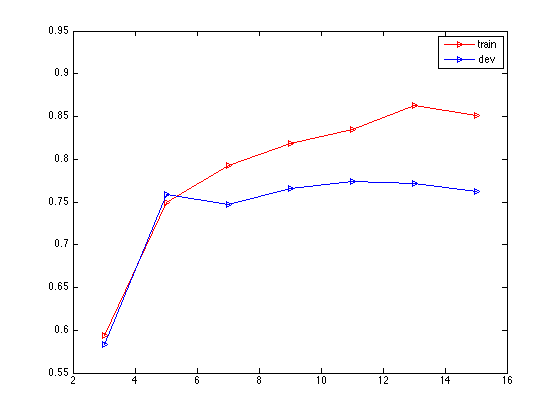
\includegraphics[scale=0.5, width=1.0\linewidth]{window.png}
  \caption{F1 score v.s. Window size $C$}
  \label{fig:window}
\end{subfigure}%
\begin{subfigure}{.5\textwidth}
  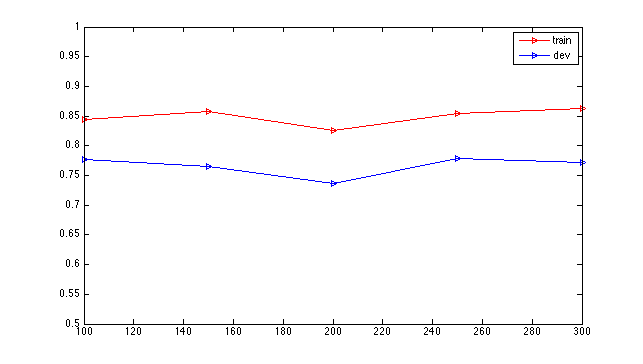
\includegraphics[scale=0.5, width=1.0\linewidth]{hidden.png}
  \caption{F1 score v.s. Single hidden layer size $H$}
  \label{fig:hidden}
\end{subfigure}
\begin{subfigure}{.5\textwidth}
  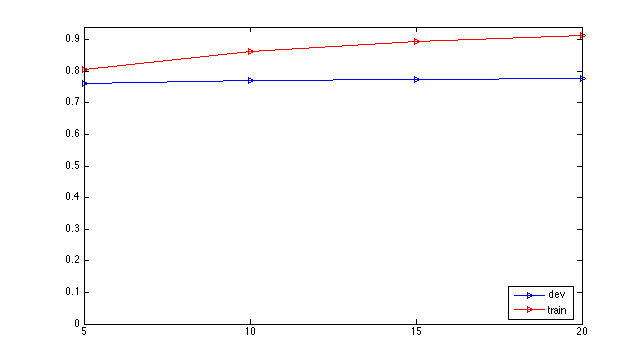
\includegraphics[scale=0.5, width=1.0\linewidth]{epoch.png}
  \caption{F1 score v.s. Epochs $K$}
  \label{fig:epoch}
\end{subfigure}%
\begin{subfigure}{.5\textwidth}
  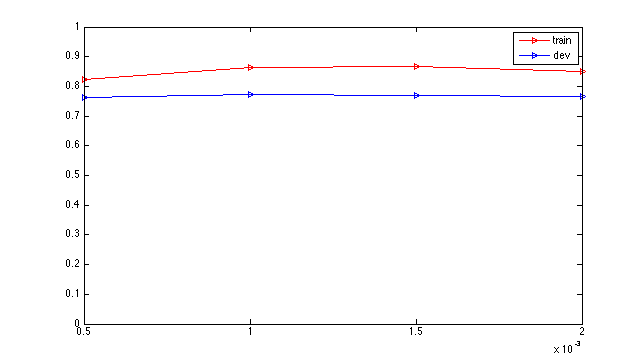
\includegraphics[scale=0.5, width=1.0\linewidth]{alpha.png}
  \caption{F1 score v.s. Learning Rate $\alpha$}
  \label{fig:alpha}
\end{subfigure}
\caption{Network parameter exploration}
\label{fig:exploration}
\end{figure}
Based on our experiments, the window size ($C$) seems to be the most influential parameter. We also observed that we seldom overfit our model throughout our exploration. The F1 score on the dev set stays between $0.75$ and $0.77$, it does not drop down even we increase our hidden layer size or the iterations. We also plot learning curves in Figure \ref{fig:learning_curve} by evaluating the cost functions after doing every $3000$ stochastic gradient descent. From this plot, we can convince ourselves that there is no need to go beyond 10 epochs because the cost function has already converged.
\begin{figure}[ht]
\begin{center}
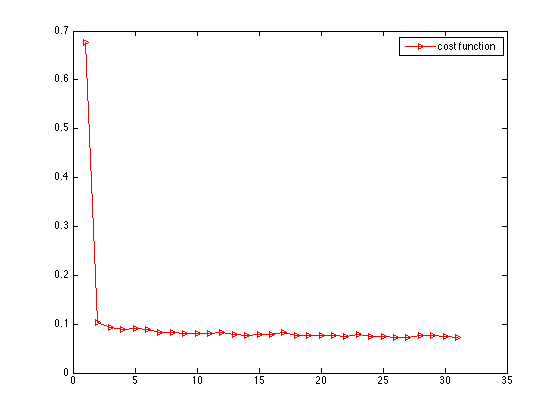
\includegraphics[width=0.5\textwidth]{curve.png}
\caption{Learning curve obtained by evaluating cost functions every $3000$ SGD iterations}
\label{fig:learning_curve}
\end{center}
\end{figure}
We summarize some of our best results from these runs in Table \ref{tab:network}.
\begin{table}[h]
\begin{center}
\begin{tabular}{|c|c|c|c|}
\hline
\multirow{2}{*}{Network Parameters} & 
\multicolumn{3}{|c|}{PERSON (training/dev)}
\\
\hhline{~---}
& Precision(\%) & Recall (\%) & F1 (\%) \\
\hline
$C$=11, $H$=300, $K$=10, $\alpha=0.001$ & 81.78/77.20 & 85.14/77.64 & 83.43/77.42
\\ \hline
$C$=13, $H$=300, $K$=5, $\alpha=0.001$ &
85.13/83.35 & 76.60/70.09 & 80.64/76.14
\\ \hline
$C$=13, $H$=250, $K$=10, $\alpha=0.001$ & 87.66/81.21 & 83.43/74.79 & \textbf{85.49/77.86} \\
\hline
\end{tabular}
\caption{F1 scores for experiments of single hidden layer architecture}
\label{tab:network}
\end{center}
\end{table}


\subsection{Word Vector Visualization}
We picked 1000 most frequent words from both PERSON and NON-PERSON set for running tSNE to embed vectors from 50 dimensional space to 2 dimensional space for visualization.
\begin{figure}[ht]
\centering
\begin{subfigure}{.5\textwidth}
  \centering
  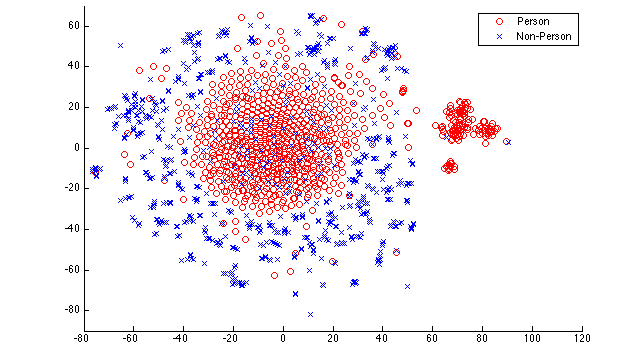
\includegraphics[width=1.0\linewidth]{before.png}
  \caption{Before training}
  \label{fig:vectors_before}
\end{subfigure}%
\begin{subfigure}{.5\textwidth}
  \centering
  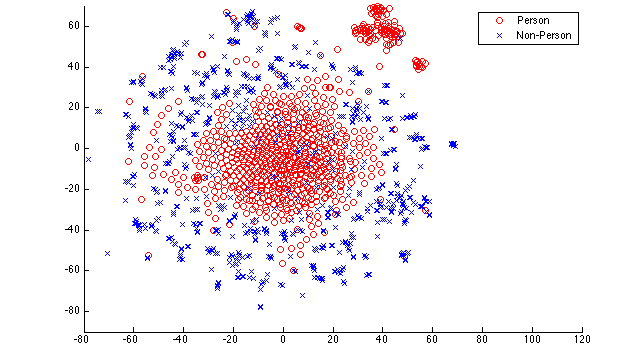
\includegraphics[width=1.0\linewidth]{after.png}
  \caption{After training}
  \label{fig:vectors_after}
\end{subfigure}
\caption{Word vector visualization}
\label{fig:vectors}
\end{figure}
The embedding algorithm shows that the initial word vectors actually perform well. Those PERSON words are approximately divided into two clusters with the larger one surrounding by those NON-PERSON words. However, we can still observe that several NON-PERSON words are mixed with those PERSON words.
After training, the larger PERSON cluster tends to be more compact than before and there are less NON-PERSON words that are mixed with PERSON words.

\subsection{Error Analysis}

\textbf{False Positive} We observe that the situations where a NON-PERSON word is recognized as a person name can be categorized as follows. The number in the parenthesis is the response score of trained neural network.
\begin{itemize}
\item Proper Noun
\begin{verbatim}
Place: Russia(0.9), Moscow(0.894), England(0.947), Texas(0.944),
Chicago(0.941), China(0.967) ...
\end{verbatim}
\begin{verbatim}
Date: Wednesday(0.953), Tuesday(0.996), September(0.897), Saturday(0.835)...
\end{verbatim}
\begin{verbatim}
Others: Honda(0.982), Mercedes-Benz(0.929), Reuters(0.841), Eurodollars(0.788),
Al(0.981), KeyCorp(0.769) ...
\end{verbatim}
\begin{verbatim}
Numbers: 6-0-40-1(0.941), 9.5-0-44-1(0.97), 42(0.92) ...
\end{verbatim}
\item Pronoun, Determinant or Preposition appear with Name
\begin{verbatim}
I(0.939), he(0.813), they(0.818), One(0.781), Some(0.643), A(0.726),
The(0.818), St(0.709), At(0.973) ...
\end{verbatim}
\item Other
\begin{verbatim}
Cardinal(0.879), Federal(0.767), Court(0.558), Commerce(0.674) ...
\end{verbatim}
\end{itemize}
For those special nouns such as brands or places, they serve a very similar purpose as a PERSON word in a sentence. We also notice some of these words are having a very high response score. It illustrates that unless with adequate domain knowledge of them, it is even hard for a real human to tell if they are a person name or not. As a PERSON name always appears with some determinant or proposition phrases, those phrases have a higher change to be misclassified as PERSON even in some NON-PERSON context. 

\vspace{0.1cm}

Generally speaking, we observe that the words that have been misclassified as person names are not random. They share both similar context and word category as person names.

\vspace{0.1cm}

\textbf{False Negative} Similar to false positive, we categorize these personal words not being recognized into:
\begin{itemize}
\item Symbol or Proposition
\begin{verbatim}
'"'(0), '('(0), ')'(0), of(0)
\end{verbatim}
\item Names
\begin{verbatim}
Clinton(0.001), Mark(0.297), Van(0.015), Albert(0.004), Dole(0.009), ...
\end{verbatim}

Due to the fact that those symbols appear more often together with NON-PERSON words, they are not recognized as person names. There are various reasons that can explain why these PERSON names are not being recognized correctly. Some names do not appear in the training set. Some names may serve other purposes in a sentence, e.g. ``Mark'' may be a verb in many cases, and ``Van'' may be a valid noun under many cases.
\end{itemize}


\section{Extra Credit and More Experiments}

\subsection{Multiple Hidden Layers}
We did some experiments to make the network deeper by specifying different hidden layer stuctures while fixing the window size ($C$) to be $13$, epoch of iterations ($K$) 5, learning rate ($\alpha$) 0.001 and regularization constant ($C$) 0.0001. Table \ref{tab:multihidden} summarizes results from these experiments.
\begin{table}[h]
\begin{center}
\begin{tabular}{|c|c|c|c|}
\hline
\multirow{2}{*}{Hidden Layer Size} & 
\multicolumn{3}{|c|}{PERSON (training/dev)}
\\
\hhline{~---}
& Precision(\%) & Recall (\%) & F1 (\%) \\
\hline
100, 100 & 82.09/80.43 & 76.47/70.50 & 79.18/75.14
\\ \hline
150, 100 & 80.83/78.10  & 79.48/72.82 & 80.15/75.37
\\ \hline
100, 150 & 78.55/76.41 & 82.49/76.34 & \textbf{80.47/76.38} \\
\hline
\end{tabular}
\caption{F1 scores for experiments of multiple hidden layers architecture}
\label{tab:multihidden}
\end{center}
\end{table}
Training deep architectures takes longer than training shallow architectures. However, training deep architectures for less number of iterations can give comparable results to shallow architectures trained with more number of iterations.


\subsection{Cut Off Point}
Observing that our data is not well-balanced, we think it makes sense to play around with the cutoff value of final response of logistic regression. In general, the recall of PERSON category is not so good given that NON-PERSON training instances outnumbers PERSON training instances.
Intuitively, we can lower the cutoff value so that the classifier will recall more PERSON instances.
Instead of using the fixed $0.5$ to determine whether a word is a person name or not, we tried to treat this cutoff as a hyperparameter and tune it on the dev set.
\begin{figure}[ht]
\begin{center}
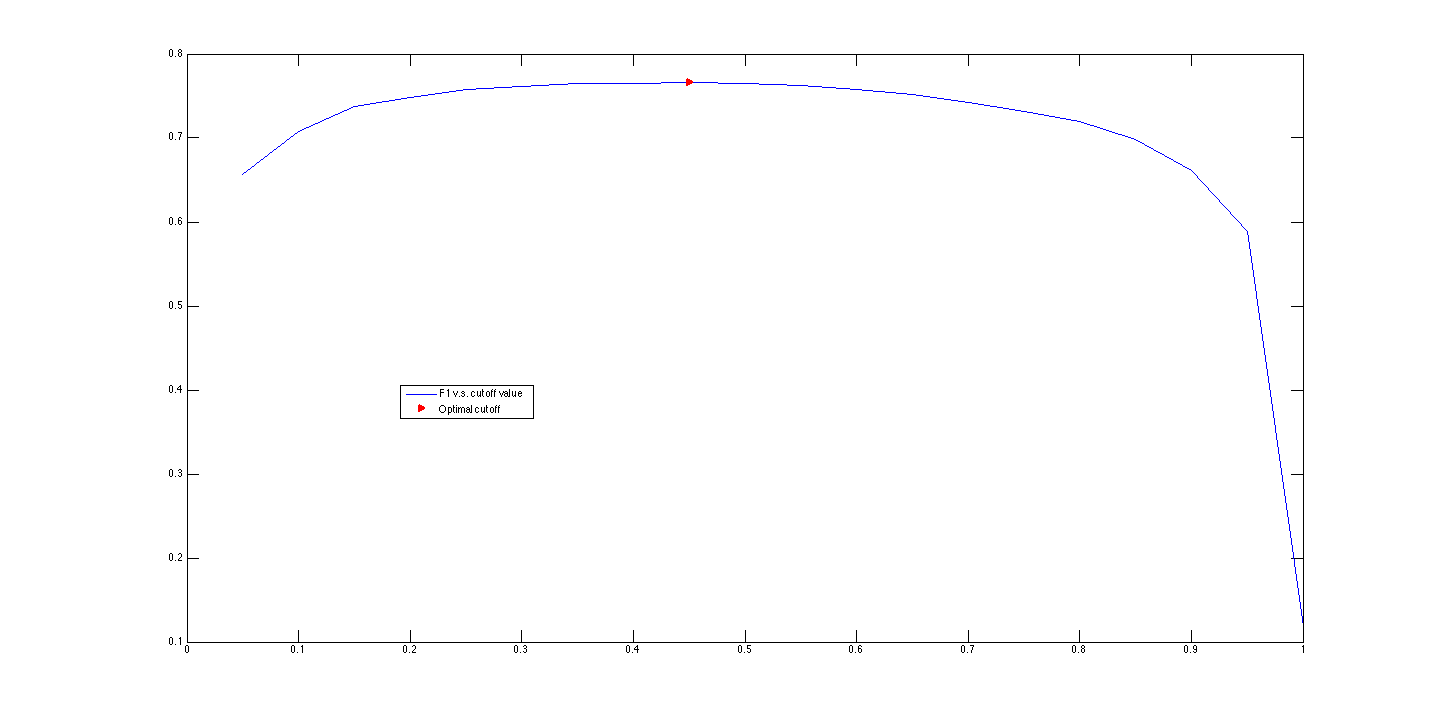
\includegraphics[scale=0.2]{f1.png}
\caption{F1 score v.s. cutoff value}
\label{fig:cutoff}
\end{center}
\end{figure}
In Figure \ref{fig:cutoff}, we vary the cutoff point from 0 to 1 with step size 0.05 and find out the best cut off value is just around 0.45 to 0.5.


\subsection{Mini-batch Gradient Descent}
We extend the SGD to a mini-batch gradient update scheme to see if we can converge to a better result in less epoch. We extend WindowModel class and override the train function to select a batch of instances.
\subsubsection{Partition}
Since there are a lot more non-person words than person words, we try to pick up a batch of instances contains both person words and non-person words together for gradient descent. We partition the training data by FIXME.
\subsubsection{Result}
The result FIXME


\end{document}